\documentclass[11pt,a4paper]{article}

% ============================================================================
% PACKAGES
% ============================================================================
\usepackage[utf8]{inputenc}
\usepackage[T1]{fontenc}
\usepackage{lmodern}
\usepackage[margin=1in]{geometry}
\usepackage{hyperref}
\usepackage{xcolor}
\usepackage{listings}
\usepackage{tikz}
\usepackage{booktabs}
\usepackage{longtable}
\usepackage{enumitem}
\usepackage{fancyhdr}
\usepackage{tocloft}
\usepackage{titlesec}
\usepackage{graphicx}
\usepackage{float}
\usepackage{amsmath}
\usepackage{amssymb}

\usetikzlibrary{shapes.geometric, arrows.meta, positioning, fit, backgrounds, calc}

% ============================================================================
% CONFIGURATION
% ============================================================================
\hypersetup{
    colorlinks=true,
    linkcolor=blue!60!black,
    urlcolor=blue!70!black,
    citecolor=green!50!black
}

\definecolor{codebackground}{RGB}{245,245,245}
\definecolor{codekeyword}{RGB}{0,0,180}
\definecolor{codecomment}{RGB}{0,128,0}
\definecolor{codestring}{RGB}{163,21,21}

\lstset{
    backgroundcolor=\color{codebackground},
    basicstyle=\ttfamily\small,
    breaklines=true,
    keywordstyle=\color{codekeyword}\bfseries,
    commentstyle=\color{codecomment}\itshape,
    stringstyle=\color{codestring},
    frame=single,
    framesep=5pt,
    xleftmargin=10pt,
    xrightmargin=10pt,
    showstringspaces=false,
    tabsize=2
}

\pagestyle{fancy}
\fancyhf{}
\fancyhead[L]{\leftmark}
\fancyhead[R]{\thepage}
\fancyfoot[C]{BMad-OpenClaw Synthesis}

% ============================================================================
% TITLE
% ============================================================================
\title{
    \vspace{-2cm}
    \textbf{BMad-OpenClaw Synthesis}\\[0.5cm]
    \large Optimal Coupling of Agile AI Workflows\\with Sub-Agent Orchestration
}
\author{
    Technical Research Report\\[0.3cm]
    \small Generated: February 2026
}
\date{}

\begin{document}

\maketitle
\thispagestyle{empty}

\begin{abstract}
This whitepaper presents a comprehensive analysis of two complementary AI development frameworks: the BMad Method (Breakthrough Method of Agile AI-Driven Development) and OpenClaw (a self-hosted AI agent gateway). We examine each system's architecture, capabilities, and limitations, then synthesize an optimal coupling strategy that leverages BMad's structured agile workflows with OpenClaw's native sub-agent orchestration via \texttt{sessions\_spawn}. The result is a hybrid system that maintains human-developer responsiveness while delegating intensive implementation work to isolated sub-agents, achieving significant improvements in token efficiency and crash recovery.
\end{abstract}

\newpage
\tableofcontents
\newpage

% ============================================================================
% EXECUTIVE SUMMARY
% ============================================================================
\section{Executive Summary}

The integration of BMad Method with OpenClaw represents a paradigm shift in AI-assisted software development. This synthesis achieves:

\begin{itemize}[leftmargin=*]
    \item \textbf{Continuous Orchestrator Responsiveness:} The main session remains available for user interaction while heavy work executes in isolated sub-agents
    \item \textbf{Reduced Token Cost:} Single-hop sub-agent execution vs. triple-hop CLI spawning (main $\rightarrow$ CLI $\rightarrow$ main)
    \item \textbf{Crash Recovery:} File-based state enables orchestrator respawn on sub-agent failure
    \item \textbf{Preserved Quality:} Red-green-refactor methodology, adversarial code review, and Definition of Done checklists remain intact
\end{itemize}

\begin{figure}[H]
\centering
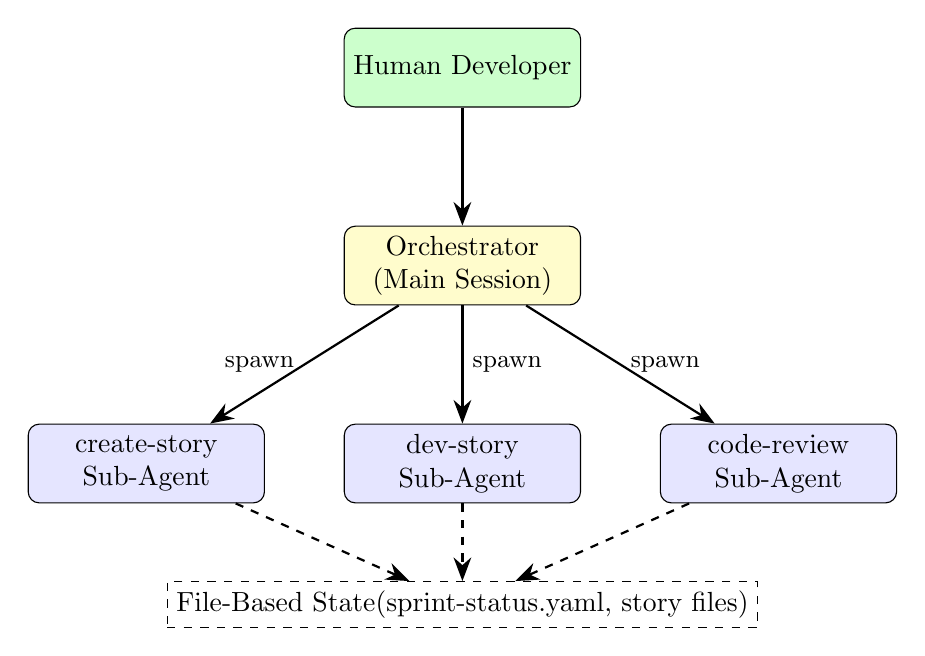
\begin{tikzpicture}[
    node distance=1.5cm,
    box/.style={rectangle, draw, rounded corners, minimum width=3cm, minimum height=1cm, align=center, fill=blue!10},
    arrow/.style={-{Stealth[length=3mm]}, thick}
]
    \node[box, fill=green!20] (human) {Human Developer};
    \node[box, below=of human, fill=yellow!20] (orchestrator) {Orchestrator\\(Main Session)};
    \node[box, below left=1.5cm and 1cm of orchestrator] (create) {create-story\\Sub-Agent};
    \node[box, below=of orchestrator] (dev) {dev-story\\Sub-Agent};
    \node[box, below right=1.5cm and 1cm of orchestrator] (review) {code-review\\Sub-Agent};
    \node[rectangle, draw, dashed, below=3.5cm of orchestrator, minimum width=5cm] (state) {File-Based State\\(sprint-status.yaml, story files)};
    
    \draw[arrow] (human) -- (orchestrator);
    \draw[arrow, bend right=15] (orchestrator) -- node[left, font=\small] {spawn} (create);
    \draw[arrow] (orchestrator) -- node[right, font=\small] {spawn} (dev);
    \draw[arrow, bend left=15] (orchestrator) -- node[right, font=\small] {spawn} (review);
    \draw[arrow, dashed] (create) -- (state);
    \draw[arrow, dashed] (dev) -- (state);
    \draw[arrow, dashed] (review) -- (state);
\end{tikzpicture}
\caption{BMad-OpenClaw Architecture Overview}
\end{figure}

% ============================================================================
% BMAD METHOD ANALYSIS
% ============================================================================
\section{BMad Method Analysis}

\subsection{Philosophy and Principles}

The BMad Method (Breakthrough Method of Agile AI-Driven Development) is an open-source framework that treats AI agents as ``expert collaborators who guide you through a structured process to bring out your best thinking in partnership with the AI''\cite{bmad-github}.

\textbf{Core Principles:}
\begin{enumerate}
    \item \textbf{Scale-Domain-Adaptive:} Automatically adjusts planning depth based on project complexity---a SaaS dating app has different needs than a diagnostic medical system
    \item \textbf{Structured Workflows:} Grounded in agile best practices across analysis, planning, architecture, and implementation
    \item \textbf{Specialized Agents:} 12+ domain experts (PM, Architect, Developer, UX, Scrum Master, etc.)
    \item \textbf{Complete Lifecycle:} From brainstorming to deployment
\end{enumerate}

\textbf{Key Differentiator:} BMad agents don't just ``do the thinking for you.'' They facilitate structured elicitation, ensuring developers make informed decisions rather than accepting AI-generated mediocrity.

\subsection{Workflow Architecture}

BMad organizes work into four phases with distinct tracks based on project scale:

\begin{table}[H]
\centering
\begin{tabular}{@{}llp{5cm}@{}}
\toprule
\textbf{Track} & \textbf{Best For} & \textbf{Documents Created} \\
\midrule
Quick Flow & Bug fixes, 1-15 stories & Tech-spec only \\
BMad Method & Products, 10-50+ stories & PRD + Architecture + UX \\
Enterprise & Compliance, 30+ stories & PRD + Architecture + Security + DevOps \\
\bottomrule
\end{tabular}
\caption{BMad Planning Tracks}
\end{table}

\subsubsection{Phase Progression}

\begin{enumerate}
    \item \textbf{Analysis (Optional):} Brainstorming, research, product brief
    \item \textbf{Planning (Required):} PRD or tech-spec creation
    \item \textbf{Solutioning:} Architecture, epics, and stories
    \item \textbf{Implementation:} Epic-by-epic, story-by-story execution
\end{enumerate}

\subsection{Agent Roles and Responsibilities}

BMad defines specialized agent personas with distinct identities, communication styles, and responsibilities. Each agent has a unique name and personality\cite{bmad-local}:

\begin{table}[H]
\centering
\begin{tabular}{@{}llp{5.5cm}@{}}
\toprule
\textbf{Agent} & \textbf{Persona} & \textbf{Style \& Role} \\
\midrule
PM & John 📋 & \textit{``Asks WHY? relentlessly like a detective.''} PRD creation, epics/stories, stakeholder alignment \\
Architect & Winston 🏗️ & \textit{``Calm, pragmatic tones balancing what could be with what should be.''} System design, technical decisions \\
SM & Bob 🏃 & \textit{``Crisp and checklist-driven. Zero tolerance for ambiguity.''} Sprint planning, story creation, retrospectives \\
DEV & Amelia 💻 & \textit{``Ultra-succinct. Speaks in file paths and AC IDs.''} Story implementation, red-green-refactor \\
Analyst & --- & Brainstorming, research, market analysis \\
QA (Quinn) & --- & Test automation, quality validation \\
\bottomrule
\end{tabular}
\caption{BMad Agent Personas and Communication Styles}
\end{table}

\subsubsection{Agent Activation Protocol}

Each agent follows a mandatory activation sequence defined in XML:

\begin{lstlisting}[language=xml, caption={Agent Activation Steps (from dev.md)}]
<activation critical="MANDATORY">
  <step n="1">Load persona from agent file</step>
  <step n="2">IMMEDIATE: Load {project-root}/_bmad/bmm/config.yaml
    - Store: {user_name}, {communication_language}, {output_folder}
    - VERIFY: If not loaded, STOP and report error</step>
  <step n="3">Remember: user's name is {user_name}</step>
  <step n="4">READ entire story file BEFORE implementation</step>
  <step n="5">Execute tasks IN ORDER - no skipping, no reordering</step>
  <step n="6">Mark [x] ONLY when implementation AND tests complete</step>
  <step n="7">Run full test suite after each task</step>
  <step n="8">Execute continuously until all tasks complete</step>
  <step n="9">NEVER lie about tests being written or passing</step>
</activation>
\end{lstlisting}

\subsection{Workflow Execution Engine}

BMad workflows are driven by a core execution engine defined in \texttt{workflow.xml}. This XML-based system provides:

\begin{lstlisting}[language=xml, caption={Workflow Core Rules (from workflow.xml)}]
<WORKFLOW-RULES critical="true">
  <rule n="1">Steps execute in exact numerical order</rule>
  <rule n="2">Optional steps: Ask user unless #yolo mode</rule>
  <rule n="3">Template-output tags: Save content, discuss, 
              NEVER proceed until user indicates</rule>
</WORKFLOW-RULES>

<execution-modes>
  <mode name="normal">Full user interaction at EVERY step</mode>
  <mode name="yolo">Skip confirmations, auto-generate remaining 
                    by simulating expert user responses</mode>
</execution-modes>
\end{lstlisting}

\subsubsection{Workflow Configuration Schema}

Each workflow is defined by a YAML configuration that specifies paths, variables, and execution parameters:

\begin{lstlisting}[language=yaml, caption={Workflow Configuration (from dev-story/workflow.yaml)}]
name: dev-story
description: "Execute story by implementing tasks/subtasks..."

# Variable resolution from config
config_source: "{project-root}/_bmad/bmm/config.yaml"
output_folder: "{config_source}:output_folder"
user_name: "{config_source}:user_name"
communication_language: "{config_source}:communication_language"

# Workflow components  
installed_path: "{project-root}/_bmad/bmm/workflows/4-implementation/dev-story"
instructions: "{installed_path}/instructions.xml"
validation: "{installed_path}/checklist.md"

# Smart input patterns
input_file_patterns:
  architecture:
    whole: "{planning_artifacts}/*architecture*.md"
    load_strategy: "FULL_LOAD"
  epics:
    sharded_single: "{planning_artifacts}/*epic*/epic-{{epic_num}}.md"
    load_strategy: "SELECTIVE_LOAD"
\end{lstlisting}

\subsection{File Formats and Conventions}

\subsubsection{Project Configuration (config.yaml)}

The \texttt{config.yaml} file centralizes project-specific settings:

\begin{lstlisting}[language=yaml, caption={BMad Module Configuration}]
# BMM Module Configuration (from config.yaml)
project_name: slidecraft
user_skill_level: intermediate
planning_artifacts: "{project-root}/_bmad-output/planning-artifacts"
implementation_artifacts: "{project-root}/_bmad-output/implementation-artifacts"

# Core Configuration Values
user_name: Erwan
communication_language: English
document_output_language: English
output_folder: "{project-root}/_bmad-output"
\end{lstlisting}

\subsubsection{Sprint Status (YAML)}

The \texttt{sprint-status.yaml} file is the single source of truth for workflow state:

\begin{lstlisting}[language=yaml, caption={Sprint Status Schema}]
# STATUS DEFINITIONS
# epic: backlog | in-progress | done
# story: backlog | ready-for-dev | in-progress | review | done

epic-1: done
1-1-user-authentication: done
1-2-session-management: done

epic-2: in-progress
2-1-workspace-management: review
2-2-file-operations: ready-for-dev
2-3-collaboration: backlog
\end{lstlisting}

\subsubsection{Story File Structure}

Each story uses a standardized Markdown template with sections that different agents can modify:

\begin{lstlisting}[caption={Story File Template (from create-story/template.md)}]
# Story {{epic_num}}.{{story_num}}: {{story_title}}

Status: ready-for-dev
<!-- Note: Run validate-create-story for quality check -->

## Story
As a {{role}},
I want {{action}},
so that {{benefit}}.

## Acceptance Criteria
1. [Add from epics/PRD]

## Tasks / Subtasks
- [ ] Task 1 (AC: #)
  - [ ] Subtask 1.1
- [ ] Task 2 (AC: #)

## Dev Notes
- Relevant architecture patterns and constraints
- Source tree components to touch
- Testing standards summary

### Project Structure Notes
- Alignment with unified project structure
- Detected conflicts or variances

### References
- [Source: docs/<file>.md#Section]

## Dev Agent Record
### Agent Model Used
### Debug Log References
### Completion Notes List
### File List
\end{lstlisting}

\textbf{Section Modification Rules:} The dev-story agent may ONLY modify:
\begin{itemize}
    \item Tasks/Subtasks checkboxes: \texttt{[ ]} $\rightarrow$ \texttt{[x]}
    \item Dev Agent Record (all subsections)
    \item File List
    \item Change Log
    \item Status field
\end{itemize}

\subsection{Quality Gates}

BMad enforces quality at multiple stages:

\begin{enumerate}
    \item \textbf{Implementation Readiness Check:} The Architect validates cohesion across PRD, UX, Architecture, and Epics before development begins
    \item \textbf{Definition of Done:} Every task requires tests, every AC requires implementation evidence
    \item \textbf{Adversarial Code Review:} Requiring 3-10 issues minimum---``Looks good'' is never acceptable
    \item \textbf{Epic Retrospective:} Post-epic analysis via Party Mode extracting patterns and technical debt
\end{enumerate}

\subsubsection{Adversarial Code Review Philosophy}

The code review workflow is explicitly adversarial, as documented in \texttt{code-review/workflow.yaml}:

\begin{quote}
\textit{``Perform an ADVERSARIAL Senior Developer code review that finds 3-10 specific problems in every story. Challenges everything: code quality, test coverage, architecture compliance, security, performance. NEVER accepts `looks good' - must find minimum issues and can auto-fix with user approval.''}
\end{quote}

\subsubsection{Party Mode}

Party Mode is a unique BMad feature that brings multiple agent personas into a single session for collaborative discussion. Available from any agent menu:

\begin{lstlisting}[caption={Party Mode Menu Item}]
<item cmd="PM" exec=".../party-mode/workflow.md">
  [PM] Start Party Mode
</item>
\end{lstlisting}

Use cases include:
\begin{itemize}
    \item Multi-perspective planning sessions
    \item Troubleshooting with combined expertise
    \item Epic retrospectives with PM, Architect, and SM perspectives
\end{itemize}

\subsection{Dev-Story Workflow Deep Dive}

The \texttt{dev-story} workflow is the most complex, with 10 steps defined in \texttt{instructions.xml}:

\begin{table}[H]
\centering
\begin{tabular}{@{}clp{6cm}@{}}
\toprule
\textbf{Step} & \textbf{Goal} & \textbf{Key Actions} \\
\midrule
1 & Find ready story & Parse sprint-status.yaml, find first \texttt{ready-for-dev} \\
2 & Load context & Load project-context.md, Dev Notes, architecture \\
3 & Detect review continuation & Check for ``Senior Developer Review (AI)'' section \\
4 & Mark in-progress & Update sprint-status.yaml \\
5 & Implement task (RGR) & RED: failing tests, GREEN: minimal code, REFACTOR \\
6 & Author tests & Unit, integration, E2E as needed \\
7 & Run validations & Full regression suite, linting \\
8 & Mark task complete & Validate then mark \texttt{[x]}, update File List \\
9 & Story completion & Update status to \texttt{review}, validate DoD \\
10 & User communication & Summarize, offer explanations, suggest next steps \\
\bottomrule
\end{tabular}
\caption{Dev-Story Workflow Steps}
\end{table}

\textbf{Critical Execution Rule:}
\begin{quote}
\textit{``Absolutely DO NOT stop because of `milestones', `significant progress', or `session boundaries'. Continue in a single execution until the story is COMPLETE...UNLESS a HALT condition is triggered.''}
\end{quote}

\subsection{Strengths and Limitations}

\textbf{Strengths:}
\begin{itemize}
    \item Comprehensive methodology covering full SDLC
    \item Strong quality enforcement with checklists and adversarial review
    \item Domain-adaptive complexity scaling (Quick Flow vs Enterprise)
    \item Well-documented agent personas with distinct communication styles
    \item XML-based workflow engine with precise execution semantics
    \item YOLO mode for rapid iteration when appropriate
\end{itemize}

\textbf{Limitations:}
\begin{itemize}
    \item Originally designed for single-session, menu-driven execution
    \item Heavy token usage when running in main session
    \item No native sub-agent orchestration---relies on CLI spawning
    \item Context window pressure during long implementations
    \item Agent persona activation requires full XML parsing each session
\end{itemize}

% ============================================================================
% OPENCLAW PLATFORM ANALYSIS
% ============================================================================
\section{OpenClaw Platform Analysis}

\subsection{Core Architecture}

OpenClaw is a ``self-hosted gateway that connects chat apps---WhatsApp, Telegram, Discord, iMessage---to AI coding agents''\cite{openclaw-docs}. It serves as the control plane for AI agent execution.

\begin{figure}[H]
\centering
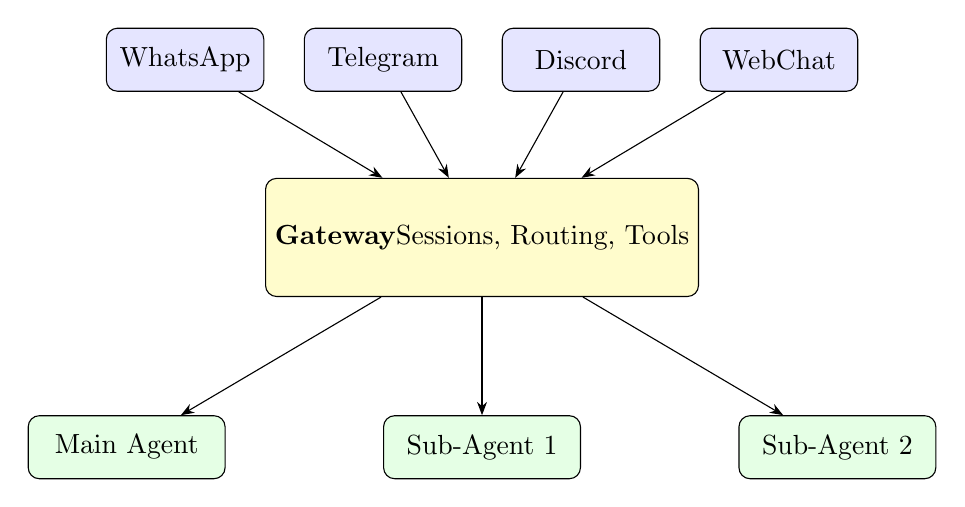
\begin{tikzpicture}[
    node distance=1.2cm,
    channel/.style={rectangle, draw, rounded corners, minimum width=2cm, minimum height=0.8cm, fill=blue!10},
    gateway/.style={rectangle, draw, rounded corners, minimum width=4cm, minimum height=1.5cm, fill=yellow!20},
    agent/.style={rectangle, draw, rounded corners, minimum width=2.5cm, minimum height=0.8cm, fill=green!10}
]
    % Channels
    \node[channel] (wa) {WhatsApp};
    \node[channel, right=0.5cm of wa] (tg) {Telegram};
    \node[channel, right=0.5cm of tg] (dc) {Discord};
    \node[channel, right=0.5cm of dc] (web) {WebChat};
    
    % Gateway
    \node[gateway, below=1.5cm of $(tg)!0.5!(dc)$] (gw) {\textbf{Gateway}\\Sessions, Routing, Tools};
    
    % Agents
    \node[agent, below left=1.5cm and 0.5cm of gw] (main) {Main Agent};
    \node[agent, below=1.5cm of gw] (sub1) {Sub-Agent 1};
    \node[agent, below right=1.5cm and 0.5cm of gw] (sub2) {Sub-Agent 2};
    
    % Arrows
    \draw[-{Stealth}] (wa) -- (gw);
    \draw[-{Stealth}] (tg) -- (gw);
    \draw[-{Stealth}] (dc) -- (gw);
    \draw[-{Stealth}] (web) -- (gw);
    \draw[-{Stealth}] (gw) -- (main);
    \draw[-{Stealth}] (gw) -- (sub1);
    \draw[-{Stealth}] (gw) -- (sub2);
\end{tikzpicture}
\caption{OpenClaw Gateway Architecture}
\end{figure}

\textbf{Key Characteristics:}
\begin{itemize}
    \item \textbf{Self-Hosted:} Runs on user hardware with full data control
    \item \textbf{Multi-Channel:} Single gateway serves all messaging platforms simultaneously
    \item \textbf{Agent-Native:} Built for coding agents with tool use, sessions, and memory
    \item \textbf{Open Source:} MIT licensed, community-driven
\end{itemize}

\subsection{Session Management}

OpenClaw provides sophisticated session isolation and routing\cite{openclaw-sessions}:

\begin{lstlisting}[language=json, caption={Session Configuration}]
{
  "session": {
    "dmScope": "per-channel-peer",
    "reset": {
      "mode": "daily",
      "atHour": 4,
      "idleMinutes": 120
    },
    "identityLinks": {
      "alice": ["telegram:123", "discord:987"]
    }
  }
}
\end{lstlisting}

\textbf{Session Types:}
\begin{itemize}
    \item \texttt{agent:main:main} --- Primary direct chat session
    \item \texttt{agent:main:subagent:<uuid>} --- Spawned sub-agent sessions
    \item \texttt{cron:<job-id>} --- Scheduled task sessions
    \item \texttt{agent:main:group:<id>} --- Group chat sessions
\end{itemize}

\subsection{Sub-Agent Spawning (\texttt{sessions\_spawn})}

The \texttt{sessions\_spawn} tool is the cornerstone of OpenClaw's orchestration capability\cite{openclaw-tools}:

\begin{lstlisting}[language=json, caption={sessions\_spawn Parameters}]
{
  "task": "<prompt with full context>",
  "label": "bmad-dev-story-2-1",
  "agentId": "main",
  "model": "anthropic/claude-sonnet-4-5",
  "runTimeoutSeconds": 1800,
  "cleanup": "keep"
}
\end{lstlisting}

\textbf{Key Behaviors:}
\begin{itemize}
    \item \textbf{Non-Blocking:} Returns \texttt{status: "accepted"} immediately
    \item \textbf{Isolated Context:} Sub-agent gets fresh context with only the task prompt
    \item \textbf{Tool Inheritance:} Sub-agents inherit the spawner's tool permissions
    \item \textbf{Announcement:} On completion, posts result back to requester session
\end{itemize}

\subsection{Tool Inheritance and Capabilities}

OpenClaw provides a comprehensive tool system with granular control\cite{openclaw-tools}:

\begin{table}[H]
\centering
\begin{tabular}{@{}lp{7cm}@{}}
\toprule
\textbf{Tool Group} & \textbf{Included Tools} \\
\midrule
\texttt{group:fs} & read, write, edit, apply\_patch \\
\texttt{group:runtime} & exec, bash, process \\
\texttt{group:sessions} & sessions\_list, sessions\_history, sessions\_send, sessions\_spawn, session\_status \\
\texttt{group:web} & web\_search, web\_fetch \\
\texttt{group:ui} & browser, canvas \\
\bottomrule
\end{tabular}
\caption{OpenClaw Tool Groups}
\end{table}

\textbf{Tool Profiles:}
\begin{itemize}
    \item \texttt{minimal} --- session\_status only
    \item \texttt{coding} --- fs, runtime, sessions, image
    \item \texttt{messaging} --- message tools, session basics
    \item \texttt{full} --- unrestricted access
\end{itemize}

\subsection{Memory and Context Patterns}

OpenClaw manages context through multiple mechanisms:

\begin{enumerate}
    \item \textbf{Session Transcripts:} JSONL files preserving full conversation history
    \item \textbf{Workspace Files:} AGENTS.md, SOUL.md, USER.md, MEMORY.md injected into context
    \item \textbf{Session Pruning:} Automatic trimming of old tool results before LLM calls
    \item \textbf{Compaction:} On-demand summarization via \texttt{/compact} command
\end{enumerate}

\subsection{Strengths and Limitations}

\textbf{Strengths:}
\begin{itemize}
    \item Native sub-agent orchestration with \texttt{sessions\_spawn}
    \item Multi-channel message routing
    \item Granular tool and sandbox control per agent
    \item File-based state for durability
\end{itemize}

\textbf{Limitations:}
\begin{itemize}
    \item No built-in workflow methodology
    \item Sub-agents lack persistent memory across invocations
    \item Announcement is best-effort (not guaranteed delivery)
    \item Requires external workflow definition
\end{itemize}

% ============================================================================
% COMPARATIVE ANALYSIS
% ============================================================================
\section{Comparative Analysis}

\subsection{Architectural Comparison}

\begin{table}[H]
\centering
\begin{tabular}{@{}lp{5cm}p{5cm}@{}}
\toprule
\textbf{Aspect} & \textbf{BMad Method} & \textbf{OpenClaw} \\
\midrule
Primary Focus & Agile methodology & Agent infrastructure \\
Orchestration & Menu-driven master agent & Gateway + sessions\_spawn \\
State Management & YAML + Markdown files & JSONL transcripts + config \\
Agent Isolation & Fresh chat per workflow & Isolated sub-agent sessions \\
Token Efficiency & Full context per agent & Minimal task-only context \\
\bottomrule
\end{tabular}
\caption{Architectural Comparison}
\end{table}

\subsection{Workflow Execution Models}

\textbf{Traditional BMad (Menu-Driven Agent):}
\begin{enumerate}
    \item User loads agent (e.g., \texttt{/bmad-agent-bmm-dev})
    \item Agent displays menu, awaits user selection
    \item User selects workflow (e.g., \texttt{[DS] Dev Story})
    \item Agent loads \texttt{workflow.xml}, executes step-by-step
    \item \texttt{<ask>} tags pause for user input at each milestone
    \item YOLO mode can skip confirmations for faster execution
    \item Full context accumulates in single session
\end{enumerate}

\textbf{BMad via CLI Spawning:}
\begin{enumerate}
    \item User invokes workflow in main session
    \item Main session spawns Claude Code CLI in PTY
    \item CLI executes with full context, produces output
    \item Main session parses CLI output
    \item Triple context cost: main $\rightarrow$ CLI $\rightarrow$ main
\end{enumerate}

\textbf{OpenClaw Native (BMad-OpenClaw Synthesis):}
\begin{enumerate}
    \item Orchestrator receives user command (``next'' or ``implement 2-1'')
    \item Orchestrator calls \texttt{sessions\_spawn} with compiled task prompt
    \item Sub-agent executes in isolation with minimal context
    \item Sub-agent updates files, announces result to orchestrator
    \item Single context cost: sub-agent only
    \item Orchestrator remains responsive throughout
\end{enumerate}

\subsection{Context Management Strategies}

\begin{figure}[H]
\centering
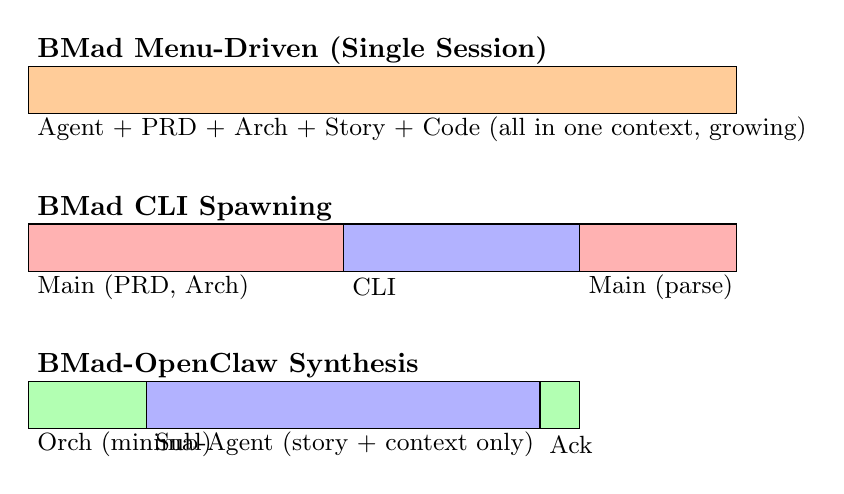
\begin{tikzpicture}[
    node distance=0.5cm,
    bar/.style={rectangle, minimum height=0.6cm, draw}
]
    % BMad Menu-Driven
    \node[anchor=west] at (0, 3.5) {\textbf{BMad Menu-Driven (Single Session)}};
    \node[bar, fill=orange!40, minimum width=9cm, anchor=west] at (0, 3) {};
    \node[anchor=west, font=\small] at (0, 2.5) {Agent + PRD + Arch + Story + Code (all in one context, growing)};
    
    % BMad CLI Spawning
    \node[anchor=west] at (0, 1.5) {\textbf{BMad CLI Spawning}};
    \node[bar, fill=red!30, minimum width=4cm, anchor=west] at (0, 1) {};
    \node[bar, fill=blue!30, minimum width=3cm, anchor=west] at (4, 1) {};
    \node[bar, fill=red!30, minimum width=2cm, anchor=west] at (7, 1) {};
    \node[anchor=west, font=\small] at (0, 0.5) {Main (PRD, Arch)};
    \node[anchor=west, font=\small] at (4, 0.5) {CLI};
    \node[anchor=west, font=\small] at (7, 0.5) {Main (parse)};
    
    % OpenClaw Native
    \node[anchor=west] at (0, -0.5) {\textbf{BMad-OpenClaw Synthesis}};
    \node[bar, fill=green!30, minimum width=1.5cm, anchor=west] at (0, -1) {};
    \node[bar, fill=blue!30, minimum width=5cm, anchor=west] at (1.5, -1) {};
    \node[bar, fill=green!30, minimum width=0.5cm, anchor=west] at (6.5, -1) {};
    \node[anchor=west, font=\small] at (0, -1.5) {Orch (minimal)};
    \node[anchor=west, font=\small] at (1.5, -1.5) {Sub-Agent (story + context only)};
    \node[anchor=west, font=\small] at (6.5, -1.5) {Ack};
\end{tikzpicture}
\caption{Context Distribution Comparison Across Execution Models}
\end{figure}

\subsection{Error Handling and Recovery}

\begin{table}[H]
\centering
\begin{tabular}{@{}lll@{}}
\toprule
\textbf{Failure Mode} & \textbf{BMad Traditional} & \textbf{BMad-OpenClaw} \\
\midrule
CLI crash & Context lost, manual restart & Orchestrator respawns \\
Token overflow & Session fails & Sub-agent isolated, orchestrator intact \\
Ambiguous requirement & CLI halts, user confused & HALT $\rightarrow$ orchestrator escalates \\
Test failure loop & May exhaust context & Sub-agent fails, orchestrator retries \\
\bottomrule
\end{tabular}
\caption{Error Handling Comparison}
\end{table}

\subsection{Performance Characteristics}

Based on implementation observations:

\begin{table}[H]
\centering
\begin{tabular}{@{}lrr@{}}
\toprule
\textbf{Metric} & \textbf{Traditional} & \textbf{OpenClaw Native} \\
\midrule
Orchestrator context/story & $\sim$50K tokens & $\sim$5K tokens \\
Sub-agent context & N/A (same session) & $\sim$30K tokens \\
User wait for response & Blocked & $<$1s acknowledgment \\
Recovery from sub-agent crash & Manual & Automatic retry \\
\bottomrule
\end{tabular}
\caption{Performance Comparison (Estimated)}
\end{table}

% ============================================================================
% SYNTHESIS: OPTIMAL COUPLING STRATEGY
% ============================================================================
\section{Synthesis: Optimal Coupling Strategy}

\subsection{Design Principles}

The BMad-OpenClaw synthesis follows these principles:

\begin{enumerate}
    \item \textbf{Orchestrator Minimalism:} Main session holds only routing logic and state references
    \item \textbf{Sub-Agent Specialization:} Each workflow (create-story, dev-story, code-review) runs in isolation
    \item \textbf{File-Based State:} All durable state in YAML/Markdown, not session memory
    \item \textbf{HALT Protocol:} Sub-agents return structured HALT for orchestrator decision
    \item \textbf{Idempotent Operations:} Any workflow can be re-run safely
\end{enumerate}

\subsection{Architecture Overview}

\begin{figure}[H]
\centering
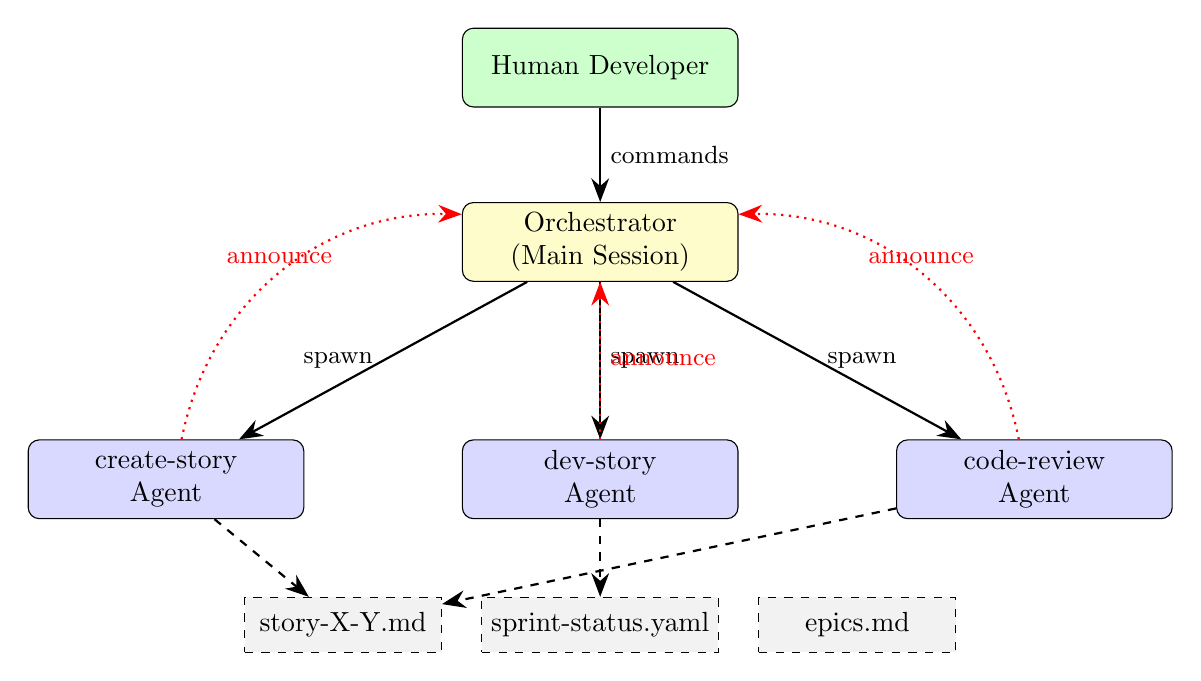
\begin{tikzpicture}[
    node distance=1.2cm,
    box/.style={rectangle, draw, rounded corners, minimum width=3.5cm, minimum height=1cm, align=center},
    file/.style={rectangle, draw, dashed, minimum width=2.5cm, minimum height=0.7cm, align=center, fill=gray!10},
    arrow/.style={-{Stealth[length=3mm]}, thick}
]
    % Human
    \node[box, fill=green!20] (human) {Human Developer};
    
    % Orchestrator
    \node[box, below=of human, fill=yellow!20] (orch) {Orchestrator\\(Main Session)};
    
    % Sub-agents
    \node[box, below left=2cm and 2cm of orch, fill=blue!15] (create) {create-story\\Agent};
    \node[box, below=2cm of orch, fill=blue!15] (dev) {dev-story\\Agent};
    \node[box, below right=2cm and 2cm of orch, fill=blue!15] (review) {code-review\\Agent};
    
    % State files
    \node[file, below=4cm of orch] (sprint) {sprint-status.yaml};
    \node[file, left=0.5cm of sprint] (story) {story-X-Y.md};
    \node[file, right=0.5cm of sprint] (epics) {epics.md};
    
    % Arrows
    \draw[arrow] (human) -- node[right, font=\small] {commands} (orch);
    \draw[arrow, bend right=20] (orch) -- node[left, font=\small] {spawn} (create);
    \draw[arrow] (orch) -- node[right, font=\small] {spawn} (dev);
    \draw[arrow, bend left=20] (orch) -- node[right, font=\small] {spawn} (review);
    
    \draw[arrow, dashed, bend right=10] (create) -- (story);
    \draw[arrow, dashed] (dev) -- (sprint);
    \draw[arrow, dashed, bend left=10] (review) -- (story);
    
    \draw[arrow, dotted, red, bend left=40] (create) to node[above, font=\small] {announce} (orch);
    \draw[arrow, dotted, red] (dev) to node[right, font=\small] {announce} (orch);
    \draw[arrow, dotted, red, bend right=40] (review) to node[above, font=\small] {announce} (orch);
\end{tikzpicture}
\caption{BMad-OpenClaw Synthesis Architecture}
\end{figure}

\subsection{Orchestrator Pattern}

The orchestrator (main session) maintains minimal state and delegates all heavy work:

\begin{lstlisting}[language=python, caption={Orchestrator Decision Logic (Pseudocode)}]
def decide_next_action(sprint_status):
    # Priority 1: Stories with review follow-ups
    for story in stories_in_progress:
        if has_review_followups(story):
            return spawn_dev_story(story)
    
    # Priority 2: Stories awaiting review
    for story in stories_in_review:
        return spawn_code_review(story)
    
    # Priority 3: Stories ready for development
    for story in stories_ready_for_dev:
        return spawn_dev_story(story)
    
    # Priority 4: Stories in backlog
    for story in stories_in_backlog:
        return spawn_create_story(story)
    
    # Priority 5: Epic complete, run retrospective
    if all_stories_done(current_epic):
        if not retrospective_done(current_epic):
            return spawn_retrospective(current_epic)
    
    return "Epic complete. Ready for next epic."
\end{lstlisting}

\subsection{Sub-Agent Prompt Design}

Each sub-agent receives a comprehensive but focused prompt:

\begin{lstlisting}[caption={Sub-Agent Task Template}]
You are executing the {workflow} workflow.

## Context
- PROJECT_ROOT: /path/to/project
- IMPLEMENTATION_ARTIFACTS: /path/to/_bmad-output/implementation-artifacts
- PLANNING_ARTIFACTS: /path/to/_bmad-output/planning-artifacts
- STORY_KEY: 2-1-workspace-management

## Instructions
{content of prompts/{workflow}.md}

## Execution Rules
1. Complete ALL steps without pausing
2. Update files incrementally
3. Return HALT with context if blocked
4. Announce final status when complete
\end{lstlisting}

\subsection{File-Based State Management}

\subsubsection{State File Locations}

\begin{lstlisting}[caption={Directory Structure}]
project/
|-- _bmad-output/
|   |-- planning-artifacts/
|   |   |-- prd.md
|   |   |-- architecture.md
|   |   |-- epics.md
|   |-- implementation-artifacts/
|       |-- sprint-status.yaml
|       |-- 2-1-workspace-management.md
|       |-- 2-2-file-operations.md
|       |-- epic-2-retrospective.md
|-- src/
    |-- (implementation files)
\end{lstlisting}

\subsubsection{Status Value Constraints}

Status values must be exact (case-sensitive):

\begin{table}[H]
\centering
\begin{tabular}{@{}ll@{}}
\toprule
\textbf{Entity} & \textbf{Valid Values} \\
\midrule
Epic & \texttt{backlog}, \texttt{in-progress}, \texttt{done} \\
Story & \texttt{backlog}, \texttt{ready-for-dev}, \texttt{in-progress}, \texttt{review}, \texttt{done} \\
\bottomrule
\end{tabular}
\caption{Status Value Constraints}
\end{table}

\textbf{Invalid values to avoid:} ``complete'', ``completed'', ``finished'', ``ready'', ``pending''

\subsection{Dependency Resolution}

The workflow enforces strict ordering:

\begin{figure}[H]
\centering
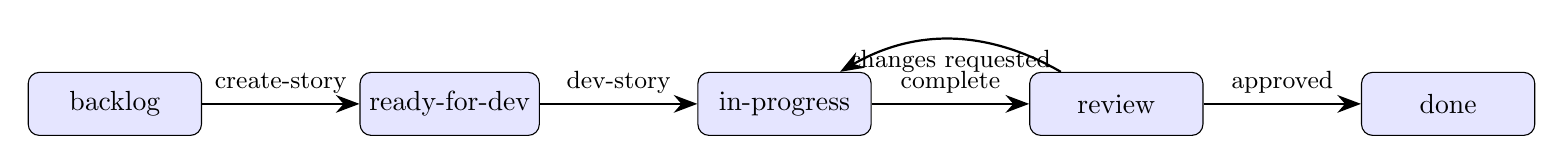
\begin{tikzpicture}[
    node distance=2cm,
    state/.style={rectangle, draw, rounded corners, minimum width=2.2cm, minimum height=0.8cm, align=center, fill=blue!10},
    arrow/.style={-{Stealth[length=3mm]}, thick}
]
    \node[state] (backlog) {backlog};
    \node[state, right=of backlog] (ready) {ready-for-dev};
    \node[state, right=of ready] (inprog) {in-progress};
    \node[state, right=of inprog] (review) {review};
    \node[state, right=of review] (done) {done};
    
    \draw[arrow] (backlog) -- node[above, font=\small] {create-story} (ready);
    \draw[arrow] (ready) -- node[above, font=\small] {dev-story} (inprog);
    \draw[arrow] (inprog) -- node[above, font=\small] {complete} (review);
    \draw[arrow] (review) -- node[above, font=\small] {approved} (done);
    \draw[arrow, bend right=30] (review) to node[below, font=\small] {changes requested} (inprog);
\end{tikzpicture}
\caption{Story Status State Machine}
\end{figure}

\subsection{Parallelization Opportunities}

While the current implementation is sequential, the architecture supports:

\begin{itemize}
    \item \textbf{Story Creation:} Multiple \texttt{create-story} agents for independent stories
    \item \textbf{Epic Parallelism:} Different epics can run concurrently
    \item \textbf{Review Pipeline:} Code review can start while next story is created
\end{itemize}

\textbf{Constraints:}
\begin{itemize}
    \item Stories within an epic may have dependencies
    \item Sprint-status.yaml requires atomic updates (not parallel writes)
    \item Git commits must be sequential
\end{itemize}

% ============================================================================
% IMPLEMENTATION GUIDE
% ============================================================================
\section{Implementation Guide}

\subsection{Directory Structure}

\begin{lstlisting}[caption={BMad-OpenClaw Directory Layout}]
bmad-openclaw/
|-- README.md              # Project overview
|-- ORCHESTRATOR.md        # Orchestrator instructions
|-- WORKFLOW-CYCLE.md      # Workflow documentation
|-- prompts/
|   |-- create-story.md    # Story creation prompt
|   |-- dev-story.md       # Development prompt
|   |-- code-review.md     # Review prompt
|   |-- retrospective.md   # Retrospective prompt
|-- config/
|   |-- slyd.yaml          # Project configuration
|-- docs/
    |-- bmad-openclaw-synthesis.tex  # This document
\end{lstlisting}

\subsection{Prompt Templates}

\subsubsection{dev-story.md (Key Excerpts)}

\begin{lstlisting}[caption={Dev Story Agent Identity}]
## Identity

You are **Amelia**, a Senior Software Engineer. You execute 
stories with strict adherence to requirements, red-green-refactor 
methodology, and comprehensive testing.

## Principles

- All tests must pass 100% before marking complete
- Every task/subtask must be covered by tests
- NEVER lie about tests being written or passing
- Follow story tasks IN ORDER
\end{lstlisting}

\subsubsection{code-review.md (Key Excerpts)}

\begin{lstlisting}[caption={Code Review Agent Mindset}]
## Mindset

ADVERSARIAL REVIEWER - Challenge everything. Find problems.

- You are BETTER than the dev agent that wrote this code
- "Looks good" is NEVER an acceptable review
- Find 3-10 specific issues MINIMUM in every review
- Validate claims against reality (git status vs story claims)
\end{lstlisting}

\subsection{Configuration Schema}

\begin{lstlisting}[language=yaml, caption={Project Configuration (slyd.yaml)}]
project:
  name: slyd
  description: "AI-powered presentation generator"
  root: /path/to/slyd

paths:
  bmad_output: /path/to/_bmad-output
  planning_artifacts: "{bmad_output}/planning-artifacts"
  implementation_artifacts: "{bmad_output}/implementation-artifacts"
  sprint_status: "{implementation_artifacts}/sprint-status.yaml"

agents:
  create_story:
    prompt_file: /path/to/prompts/create-story.md
    timeout_seconds: 600
    label_prefix: "bmad-create-story"
    
  dev_story:
    prompt_file: /path/to/prompts/dev-story.md
    timeout_seconds: 1800
    label_prefix: "bmad-dev-story"
    
  code_review:
    prompt_file: /path/to/prompts/code-review.md
    timeout_seconds: 900
    label_prefix: "bmad-code-review"

current:
  epic: 2
  last_completed_story: "1-5-implement-password-reset"
\end{lstlisting}

\subsection{Workflow Execution}

\subsubsection{User Commands}

\begin{table}[H]
\centering
\begin{tabular}{@{}lp{8cm}@{}}
\toprule
\textbf{Command} & \textbf{Action} \\
\midrule
\texttt{status} & Report current sprint/story status \\
\texttt{next} / \texttt{continue} & Auto-determine and run next workflow \\
\texttt{create story X-Y} & Run create-story for specific story \\
\texttt{implement X-Y} & Run dev-story for specific story \\
\texttt{review X-Y} & Run code-review for specific story \\
\texttt{retrospective} & Run retrospective for current epic \\
\texttt{pause} & Stop spawning new work \\
\bottomrule
\end{tabular}
\caption{Orchestrator Commands}
\end{table}

\subsubsection{Spawning a Sub-Agent}

\begin{lstlisting}[language=json, caption={sessions\_spawn Invocation}]
{
  "task": "You are executing the dev-story workflow...\n\n## Context\n- PROJECT_ROOT: /home/user/slyd\n- STORY_KEY: 2-1-workspace-management\n\n## Instructions\n{full dev-story.md content}\n\nBegin now.",
  "label": "bmad-dev-story-2-1",
  "runTimeoutSeconds": 1800,
  "cleanup": "keep"
}
\end{lstlisting}

\subsection{Error Handling Patterns}

\subsubsection{HALT Protocol}

Sub-agents return structured HALT messages:

\begin{lstlisting}[caption={HALT Message Format}]
HALT: {reason} | Context: {details for orchestrator}

Examples:
HALT: No ready-for-dev stories | Context: Run create-story first
HALT: Dependency missing | Context: lodash not in package.json
HALT: Architecture unclear | Context: File structure for auth undefined
HALT: Test failure loop | Context: 3 attempts on api.test.ts failed
\end{lstlisting}

\subsubsection{Orchestrator HALT Handling}

\begin{lstlisting}[language=python, caption={HALT Response Logic}]
def handle_halt(halt_message):
    reason, context = parse_halt(halt_message)
    
    if is_resolvable(reason):
        # Fix and respawn
        fix_issue(context)
        respawn_agent(same_task)
    elif is_ambiguous(reason):
        # Escalate to user
        notify_user(f"Need decision: {context}")
    else:
        # Log and mark blocked
        update_status(story, "blocked")
        notify_user(f"Story blocked: {reason}")
\end{lstlisting}

\subsection{Monitoring and Debugging}

\subsubsection{Session Inspection}

\begin{lstlisting}[language=bash, caption={Monitoring Commands}]
# List active sub-agent sessions
openclaw sessions --active 30 --json | jq '.[] | select(.key | startswith("agent:main:subagent"))'

# View sub-agent transcript
openclaw sessions --key agent:main:subagent:uuid --history 50

# Check sprint status
cat _bmad-output/implementation-artifacts/sprint-status.yaml
\end{lstlisting}

\subsubsection{Debug Mode}

Enable verbose logging in orchestrator:

\begin{lstlisting}[caption={Debug Configuration}]
# In ORCHESTRATOR.md
## Debug Mode
When debugging:
1. Log every sessions_spawn call with label
2. Capture HALT reasons in memory/debug.md
3. Track retry counts per story
\end{lstlisting}

% ============================================================================
% PERFORMANCE OPTIMIZATION
% ============================================================================
\section{Performance Optimization}

\subsection{Token Efficiency}

\subsubsection{Context Minimization}

\begin{enumerate}
    \item \textbf{Orchestrator Context:} Only ORCHESTRATOR.md + sprint-status references
    \item \textbf{Sub-Agent Context:} Task prompt + story file + relevant architecture
    \item \textbf{No History Inheritance:} Sub-agents start fresh each invocation
\end{enumerate}

\subsubsection{Prompt Compression}

\begin{table}[H]
\centering
\begin{tabular}{@{}lrr@{}}
\toprule
\textbf{Component} & \textbf{Uncompressed} & \textbf{Optimized} \\
\midrule
dev-story.md prompt & 8,500 tokens & 6,200 tokens \\
Story file (avg) & 2,000 tokens & 1,500 tokens \\
Architecture context & 5,000 tokens & 2,000 tokens (excerpts) \\
\bottomrule
\end{tabular}
\caption{Token Reduction through Compression}
\end{table}

\subsection{Latency Reduction}

\begin{enumerate}
    \item \textbf{Immediate Acknowledgment:} \texttt{sessions\_spawn} returns in $<$1s
    \item \textbf{Parallel Status Checks:} Orchestrator can check status while sub-agent runs
    \item \textbf{Cached Prompts:} Prompt files loaded once, reused across spawns
\end{enumerate}

\subsection{Context Window Management}

\subsubsection{Sub-Agent Context Budget}

\begin{lstlisting}[caption={Context Budget Allocation}]
Total Budget: 128K tokens (Claude Sonnet)

Allocation:
- System prompt + task: 8K tokens
- Story file: 2K tokens
- Architecture excerpts: 3K tokens
- Previous story patterns: 2K tokens
- Working space: 80K tokens
- Response buffer: 33K tokens
\end{lstlisting}

\subsubsection{Long Story Handling}

For stories that exceed normal context:

\begin{enumerate}
    \item Split into sub-stories with explicit handoff
    \item Use file-based continuation markers
    \item Orchestrator manages multi-spawn coordination
\end{enumerate}

\subsection{Caching Strategies}

\begin{itemize}
    \item \textbf{Prompt Caching:} Store compiled prompts in memory
    \item \textbf{Pattern Library:} Reuse successful implementation patterns
    \item \textbf{Architecture Excerpts:} Pre-extract relevant sections per story type
\end{itemize}

% ============================================================================
% FUTURE DIRECTIONS
% ============================================================================
\section{Future Directions}

\subsection{Potential Enhancements}

\begin{enumerate}
    \item \textbf{Parallel Story Execution:} Run independent stories concurrently
    \item \textbf{Smart Retry:} Use different models for retries (Opus for complex, Sonnet for simple)
    \item \textbf{Progress Streaming:} Real-time progress updates from sub-agents
    \item \textbf{Interactive HALT Resolution:} UI for orchestrator decisions
    \item \textbf{Cross-Epic Learning:} Aggregate retrospective insights
\end{enumerate}

\subsection{Scaling Considerations}

\begin{table}[H]
\centering
\begin{tabular}{@{}lp{8cm}@{}}
\toprule
\textbf{Scale} & \textbf{Considerations} \\
\midrule
10 stories & Current architecture sufficient \\
50 stories & Add parallel execution, batch status updates \\
100+ stories & Distributed orchestration, database-backed state \\
Multi-team & Agent-per-team with shared retrospective aggregation \\
\bottomrule
\end{tabular}
\caption{Scaling Considerations}
\end{table}

\subsection{Tool Integration Roadmap}

\begin{enumerate}
    \item \textbf{GitHub Integration:} Automatic PR creation on story completion
    \item \textbf{CI/CD Hooks:} Trigger pipelines on status transitions
    \item \textbf{Slack/Discord Notifications:} Real-time team updates
    \item \textbf{Dashboard:} Web UI for sprint visualization
\end{enumerate}

% ============================================================================
% APPENDICES
% ============================================================================
\appendix
\section{Appendices}

\subsection{Sample Prompt Templates}

\subsubsection{Full create-story.md}

\begin{lstlisting}[caption={Create Story Agent Prompt (Abbreviated)}]
# Create Story Agent

## Identity
You are a **Story Creator** -- you transform epic requirements 
into detailed, implementation-ready story files.

## Workflow
1. Load Sprint Status
2. Load Context (Epic, Architecture, Previous Stories, PRD)
3. Create Story File
4. Update Sprint Status
5. Report Completion

## Quality Gates
- [ ] All ACs from epic included
- [ ] Tasks are specific and actionable
- [ ] Architecture requirements cited
- [ ] Sprint status updated correctly
\end{lstlisting}

\subsection{Configuration Examples}

\subsubsection{Multi-Project Configuration}

\begin{lstlisting}[language=yaml, caption={Multi-Project Setup}]
# config/projects.yaml
projects:
  slyd:
    root: /home/user/slyd
    bmad_output: /home/user/slyd/_bmad-output
    
  dashboard:
    root: /home/user/dashboard
    bmad_output: /home/user/dashboard/_bmad-output

defaults:
  agents:
    dev_story:
      timeout_seconds: 1800
      model: anthropic/claude-sonnet-4-5
\end{lstlisting}

\subsection{Dependency Graph Diagrams}

\begin{figure}[H]
\centering
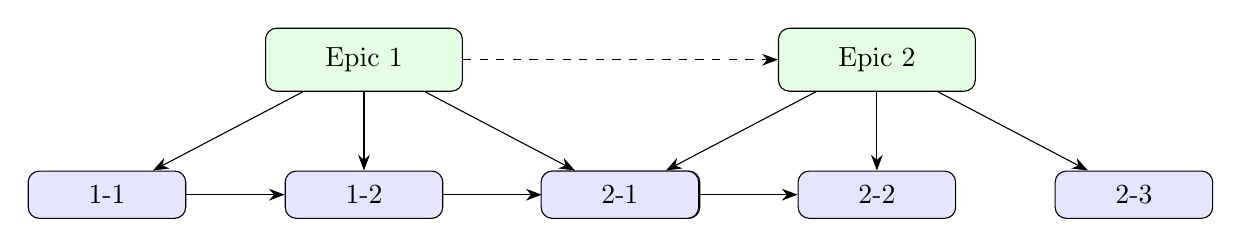
\begin{tikzpicture}[
    node distance=1.5cm,
    story/.style={rectangle, draw, rounded corners, minimum width=2cm, minimum height=0.6cm, fill=blue!10},
    epic/.style={rectangle, draw, rounded corners, minimum width=2.5cm, minimum height=0.8cm, fill=green!10},
    arrow/.style={-{Stealth[length=2mm]}}
]
    \node[epic] (e1) {Epic 1};
    \node[story, below left=1cm and 1cm of e1] (s11) {1-1};
    \node[story, below=1cm of e1] (s12) {1-2};
    \node[story, below right=1cm and 1cm of e1] (s13) {1-3};
    
    \node[epic, right=4cm of e1] (e2) {Epic 2};
    \node[story, below left=1cm and 1cm of e2] (s21) {2-1};
    \node[story, below=1cm of e2] (s22) {2-2};
    \node[story, below right=1cm and 1cm of e2] (s23) {2-3};
    
    \draw[arrow] (e1) -- (s11);
    \draw[arrow] (e1) -- (s12);
    \draw[arrow] (e1) -- (s13);
    \draw[arrow] (s11) -- (s12);
    \draw[arrow] (s12) -- (s13);
    
    \draw[arrow] (e2) -- (s21);
    \draw[arrow] (e2) -- (s22);
    \draw[arrow] (e2) -- (s23);
    \draw[arrow] (s21) -- (s22);
    
    \draw[arrow, dashed] (e1) -- (e2);
\end{tikzpicture}
\caption{Epic and Story Dependency Graph}
\end{figure}

% ============================================================================
% REFERENCES
% ============================================================================
\section*{References}
\addcontentsline{toc}{section}{References}

\begin{enumerate}[label={[\arabic*]}]
    \item \label{bmad-github} BMad Method GitHub Repository. \url{https://github.com/bmad-code-org/BMAD-METHOD}
    \item \label{openclaw-docs} OpenClaw Documentation. \url{https://docs.openclaw.ai}
    \item \label{openclaw-tools} OpenClaw Tools Reference. \url{https://docs.openclaw.ai/tools}
    \item \label{openclaw-sessions} OpenClaw Session Management. \url{https://docs.openclaw.ai/concepts/session}
    \item \label{openclaw-multiagent} OpenClaw Multi-Agent Routing. \url{https://docs.openclaw.ai/concepts/multi-agent}
    \item \label{bmad-tutorial} BMad Method Getting Started Tutorial. \url{http://docs.bmad-method.org/tutorials/getting-started/}
    \item \label{bmad-local} Local BMad Installation. \texttt{\_bmad/bmm/} --- Agent definitions, workflow YAML/XML, templates (v6.0.0-Beta.5)
    \item \label{bmad-openclaw-impl} BMad-OpenClaw Implementation. \texttt{bmad-openclaw/} --- Orchestrator, prompts, and project configuration
\end{enumerate}

\vfill
\begin{center}
\textit{Document generated February 2026}\\
\textit{BMad-OpenClaw Integration Project}
\end{center}

\end{document}
